\documentclass[12pt]{article}
\usepackage[paper=letterpaper, left=1in, right=1in, top=1in, bottom=1in]{geometry}

\usepackage[parfill]{parskip}
\usepackage{amsmath}
\usepackage{graphicx}

\begin{document}
\thispagestyle{empty}

\begin{center}
{\large CS 310}\\
Assignment 210
\end{center}

\begin{flushright}
Hieu Le
\end{flushright}

Program 210 implements an algorithm to determine the largest integral
power of 2 smaller than or equal to an arbitrary non-negative
integer. It does so by iteratively clearing the least significant set bit 
in the binary representation of the formal parameter $n$ until $n$ reaches 0. 
The last positive value of n - which is memoized in another variable i - 
before the termination of the loop gives the largest power of 2 not exceeding 
n. The algorithm will return an error value of 0 if 0 is input. This is 
unfortunate since C++ does not offer a positive integer type. 

To analyze this algorithm, we choose the assignment statement on line 26 and 33 as the basic operation as it represents the most intrinsic step of this procedure
that is also atomic and indivisible. Furthermore, compared with other statements 
in the program, it is presumably the most computationally intensive.

The value for $n$ is taken to be unsigned because inputting a negative number 
will produce an erroneous result, which should not even exist in the first
place since the procedure does not make sense for non-positive integers 
(including 0).

An empirical analysis of running the algorithm for multiple values of
$n$ produces the results shown below.

\begin{center}
\scalebox{.5} {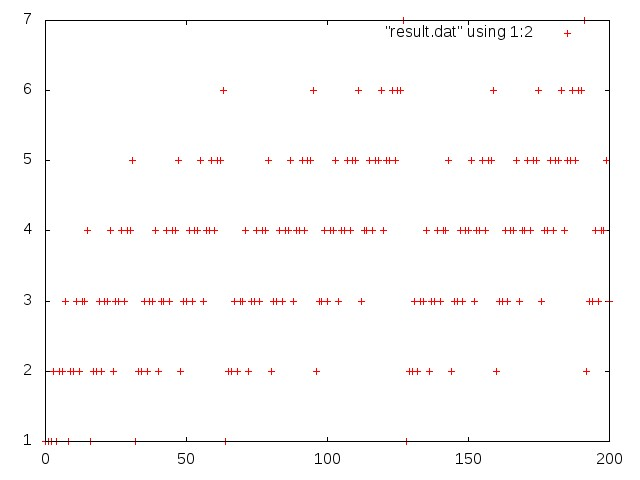
\includegraphics{plot.jpeg}}
\end{center}

An analysis of the code itself explains the empirical results when we
observe that the number of basic operations, $T(n)$, is linearly related to 
the number of set bits in the binary representation of $n$. There is no 
direct correlation between $T(n)$ and $n$ except for perhaps the observation
that as $n$ grows larger, $T(n)$ seems to fluctuate more drastically. Indeed, 
the larger $n$ is, the larger the maximum possible value of $T(n)$ is since 
the expected number of set bits in $n$ is higher. Assume that n is strictly 
positive, $T(n)$ is bounded from below by $1$ and from above by the total 
number of bits in the binary representation of $n$ - 
$\left \lfloor {log_2n} \right \rfloor$ where the floor function 
$\left \lfloor {x} \right \rfloor$ denotes the greatest integer not exceeding x.

Therefore, we conclude that this algorithm is described by

\[
T(n) \in \Omega( 1 ) \land T(n) \in O(\left \lfloor {log_2n} \right \rfloor)
\]

\end{document}
